\documentclass[a4paper]{article}
\usepackage[english]{babel}
\usepackage{subfigure,graphicx,amssymb,algorithmic,algorithm}
\graphicspath{{../figures/}}

\begin{document}
\begin{center}
Specialized Master Embedded Systems ~~\hfill Year 2010-201\\
\vspace{.3cm}
{\large \bf Hybrid Systems\\
 Lab class - Stateflow\\
}
C. Lesire \& F. Defay, October 12th, 2010
\end{center}
\vspace{.1cm}
\hrule
\vspace{.2cm}
{\bf Goal of this lab class}:
Model and simulate a hybrid system using Simulink and Stateflow.
\tableofcontents

%%% INTRODUCTION %%%
\section{A {\it Hybrid} control of a platform by a satellite's reaction wheel}

\subsection{Introduction}

Let us considerer the attitude control of a satellite with respect to a defined frame of reference,
here its gravity center. From a reference attitude  and sensor measurements of the current
attitude, a control algorithm commands the actuators that apply the torques needed to put the
satellite to the desired attitude.
In a satellite with 3 axes, the attitude control is realized using:
\begin{itemize}
\item a star tracker for the attitude measurement (the gravity center of the satellite);
\item 3 gyro-meters for the angular speed measurement and the estimated attitude (angular speed $>$ 0.1$^o$);
\item 3 reaction wheels to apply torques to the platform;
\item 3 magneto torquers (used to reduce wheels speed).
\end{itemize}

%In the \emph{Real time control of a space system EM461} course, the goal was to implement an attitude control realizing the attitude control itself and the communication with a ground station (reading current sensors values in order to output them in the ground station, do a calibration).
The following tasks have already been realized:
\begin{itemize}
\item the design of the different control laws to control the platform, to simulate them and 
to complete the C-code provided;
\item the design of the embedded software considering the temporal constraints and the 
different tasks (to manage request, to manage law and setpoint, to acquire curves information, 
to manage duration and periods).
\end{itemize}

\subsection{System Description}

The components of this platform are:
\begin{itemize}
\item a moving platform around one axe;
\item a reaction wheel driven by a DC motor;
\item the following sensors:
	\begin{itemize}
	\item 1 platform angular speed sensor;
	\item 1 motor speed sensor (tachometer);
	\item 1 absolute angular position sensor of the platform;
	\item 1 sensor measuring the motor current;
	\end{itemize}
\item a computer embedded in the satellite for executing the command laws.
\end{itemize}

\subsection{Specification}
\label{spec}

The goal is to design a (hybrid) attitude control considering only the control laws; the
communication between the satellite and the ground station \emph{is not taken into account}.
The attitude control must consider different modes according with some conditions: speed sensor
failure, eclipse occurrence, error value, etc. We consider in this project a platform representing
only one satellite's axe.

Simulink and Stateflow will be used to model and to simulate the control algorithm, 
to generate the code that will be embedded in the satellite and also to execute this 
embedded code in the target using xPC Target\footnote{xPC Target provides a high-performance 
host-target environment that enables to connect Simulink and Stateflow models to physical 
systems and execute them in real time on low-cost PC-compatible hardware. xPC Target 
includes proven capabilities for rapid prototyping, hardware-in-the-loop testing, and 
application deployment in an open hardware architecture (Mathworks).}.

As the communication with the ground station is not taken into account at this phase of 
the project, it is necessary to simulate in the Matlab environment the followings signals 
(see also section~\ref{model} and the interface in fig.~\ref{satel}(a) that will be provided in 
the skeleton of your attitude controller): PowerOn/PowerOff,  Speed Sensor OK/ Speed Sensor KO 
and the reference (setpoint).

\begin{figure}[!p]
\begin{center}
	\subfigure[Interface]{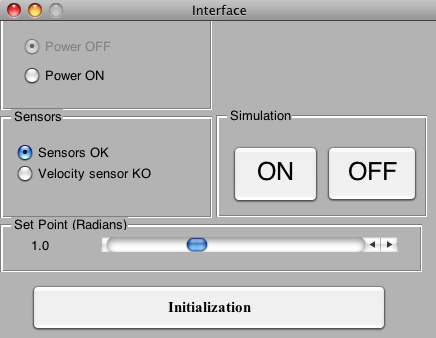
\includegraphics[width=.4\linewidth]{interfaceBEroue}}\quad
	\subfigure[Simulink block diagram]{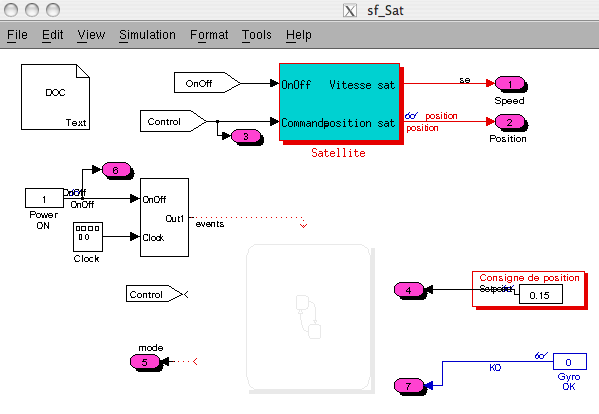
\includegraphics[width=.5\linewidth]{simulink}}\\
	\subfigure[Satellite block diagram]{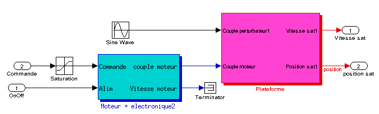
\includegraphics[width=.45\linewidth]{sat}}\quad
	\subfigure[Platform model]{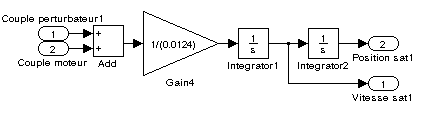
\includegraphics[width=.45\linewidth]{platef}}\\
	\subfigure[Motor\&Elec. part]{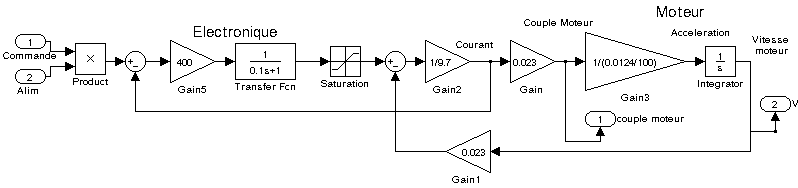
\includegraphics[width=.9\linewidth]{elec}}\\
	\subfigure[P controler]{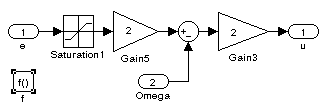
\includegraphics[width=.23\linewidth]{P}}\quad
	\subfigure[PI controler]{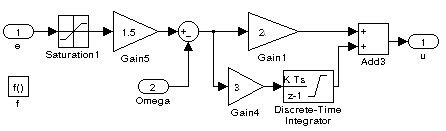
\includegraphics[width=.45\linewidth]{PI}}\quad
	\subfigure[Speed estimator]{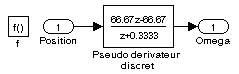
\includegraphics[width=.23\linewidth]{pseudo}}
\caption{The Simulink skeleton model provided}
\label{satel}
\end{center}
\end{figure}

The control algorithm to be implement is the following: in the initial state of the attitude 
control system, the power is off and so the attitude control 
$u$ has the initial value $0$. At the rising edge (power is On), the control system is activated. 
The control law to be used is a function of the position and the speed as before, but you must 
consider the state of the sensor (failure or not) and the degree of magnitude of the position 
error (big or small):
\begin{itemize}
\item if the position error is big (for example, abs(error) $>$ 0.1), the control law is a
proportional controller; otherwise (if the position error is small) a proportional-integral 
controller must be used. A P controller allows to lead the system quickly to the reference attitude 
when the error is big; the PI controller insures a good precision and it is used only when the 
error is small;
\item if there is an angular speed sensor failure, instead of using the angular speed value, it is 
necessary to estimate the speed from the position sensor value using a pseudo derivation.
\end{itemize}

The following algorithms/models will be provided in the skeleton of your attitude controller:
\begin{itemize}
\item the platform model (see fig.~\ref{satel}(d)),   
\item the motor and electronic model (see fig.~\ref{satel}(e)),
\item the angular speed estimator from the position sensor (see fig.~\ref{satel}(h)),
\item the P and PI controllers (see fig.~\ref{satel}(f) and (g)) and 
	the pseudo derivative estimator.
\end{itemize}

If the power is turned Off, the system comes back to an inactive state where the attitude 
control $u$ is $0$ again, independently of the error value and/or the sensor failure.

\section{Modeling the hybrid control}

You must model the hybrid control system (the different discrete states (or modes) and 
the different continuous equations), using Simulink/Stateflow (see appendix \ref{getStart} 
for a quick user guide).
It is necessary to use the Interface (provided in the skeleton) allowing to simulate in the 
Matlab environment the followings signals (see fig.~\ref{satel}(a)):
\begin{itemize}
\item PowerOn/PowerOff: is a boolean signal whose initial state is PowerOff;
\item buttons ON and OFF, for starting and stopping the control simulation or the control execution;
\item a setpoint (in radians) for changing the reference attitude;
\item an Initialization button that you need to click \emph{before} you start your simulation or execution;
\item Speed Sensor OK/ Speed Sensor KO : a boolean signal with SpeedKO=1 if there is a sensor failure and SpeedKO=0 if the sensor is working well.
\end{itemize}

To help you progress in the controler design, the lab is decomposed in several steps. Please, save
your models at each step using different names to get a trace of your progress.

\subsection{PowerOn/PowerOff transition}
First, consider the PowerOn/PowerOff signal. Write a StateFlow model with two states representing
the fact that the control is either On or Off. In the 'Off' state, the control mist be set to $0$.
In the 'On' state, the considered control law is for the moment the P controller.

\paragraph{Creating your Stateflow:}
\begin{itemize}
\item Download file {\tt BE\_Sat.zip} from {\tt Public/DISTRIB/defay} in your folder;
	there are 2 folders, {\bf sf\_Sat} for simulation and {\bf sf\_cible} for execution. 
\item Open Matlab; define the active directory as {\tt sf\_Sat}, run {\tt interface\_simu.m}:
	there are the Simulink blocks of fig.~\ref{satel};% write down the equations describing it;
\item Create a new stateflow model:
	\begin{itemize}
	\item Menu View/Simulink Library (icon 
\includegraphics[width=.5cm]{iconLib});
	\item double-click on block "Blocksets \& Toolboxes";
	\item double-clik on block Stateflow (SF); 
	\item drag a Chart block in the mdl file and change the name it; 
	\item double-click in the block to create a Stateflow model.
	\end{itemize}
\item Create your states draging the first icon on the left top to the Stateflow window; 
	replace the "?" by the state name;
\end{itemize}

You need to define the \emph{outputs} of your SF as well the \emph{inputs}, 
the \emph{state actions} and the \emph{trigger conditions}:
\begin{enumerate}
\item from the Add menu, select Data/Output from Simulink (select General tab); in the Name field,
	choose the name of your output $O$; in the Type field, select the data type;%(see 3-13).
\item you can see in the Simulink model (by clicking the icon up-arrow in the Stateflow Editor)
	that the output $O$ appear in the SF block;
\item connect the output of the SF block to the satellite model;%(3-16).
	save your model with a suffix "Equations";
\item define state actions: open your file XXX\_ Equations, click after the last letter of the
	state name, press the Enter key and type your equations and functions call (Simulink Fcn given,
	see next step);
\item open the  provided Stateflow model; there are 3 {\tt Fcn functions}: P and PI controllers and 
	speed estimator. copy each {\tt Fcn function} in the state where it is called;
	save your model with a suffix "Trans";
\item create your transitions: open you file XXX\_Trans, put the mouse on the border of the source
	state and drag the transition to the target state;% (see 6-15);
	click on each transition (it will become red), then click next to the question mark "?" and
	type the name of the event;% (6-15);
\item add a default transition in the initial state;% (see 6-8); 
	save it as XXX\_Event;
\item define edge-triggered events: open file XXX\_Event; in the Stateflow editor, Add Menu, 
	select Event/Input from Simulink;% (see 6-13). 
	define each event in the order they enter in the mux block of the satellite model (2 events,
	see fig.~\ref{satel}(b)); you don't need to use the same names, only the order in the mux is
	important; let the Trigger "Rising", "Either" or "Falling"; using the up-arrow icon, verify
	that there is a trigger symbol in the SF; save the model as XXX\_Trig;
\item connect the edge-triggered events to the input signals:% (see 7-4): 
	open XXX\_Trig file; in the Simulink window, connect the mux output to the trigger input of 
	the SF;
\item if there is no errors, you can now simulate your hybrid model. Have fun!
\end{enumerate}

Save the model and simulate it (see sec. \ref{simu}) to verify its behavior.

\subsection{Position error}
Consider now the position error. Depending on the magnitude of this error, the control law must
be either a P or a PI controler.

\subsection{Speed sensor failure}
Consider now that the speed sensor can fail. In that case, you should use the speed estimator
in addition to the controler used depending on the position error value.

\subsection{Remarks on Stateflow execution}

The stateflow is awaken at each event occurrence (rising or falling edge) or at some sampling 
frequency, given by the clock block of simulink. The continuous functions executed in a state can 
need a particular sampling frequency. For example, the sensor must be sampled ($T_s=0.01s$) and the 
control laws must be calculated at the same frequency. There are two ways to do this: choosing a 
fixed step solver for Simulink or put a self-transition in this state with an event \texttt{clock} 
as a label.

\section{Simulating your Stateflow}
\label{simu}

Two scopes to analyze your input and output signals are already in the provided skeleton.
To connect a signal, right click on its line and choose {\tt Connect to Existent Viewer}.

Suggestion: put in the scopes the attitude control, PowerOn/PowerOff, SensorKO, position, setpoint. 
Put in a same scope signals that have roughly the same magnitude.\\

At each simulation:
\begin{enumerate}
\item click on the Initialization button in the Interface window (fig.~\ref{satel}(a));
\item enter a new set of input signals allowing you to really test several configurations for
	validate your model by simulation; Remember that the simulation is not exhaustive, and a good
	{\it set} of input values are a key for the model validation; try to start testing the most
	important cases;
\item the simulation will stop after 20s with the provided skeleton; you can change it if you want;
\item if you click on the scope after the simulation is finished, sometimes the scale is to big
	due to the maximal values; you can type the command line {\tt trace\_sim} on the Matlab window
	(command window) to better see the simulating results.
\end{enumerate}

\section{Executing your Stateflow on the target}

The Stateflow will be compiled and run on the target (embedded in the satellite).
At this step, the satellite is no more simulated (as in  fig.~\ref{satel}(b) to 
fig.~\ref{satel}(d)) but will receive the control generated by the stateflow and provide the 
inputs for it.% The new Simulink bloc diagram is depicted in fig.~\ref{target}.

When using Matlab for simulation, the model run directly on the PC under development.
When using xPC Target, the Simulink model is compiled and loaded in the XPC target in real time. 
The PC is connected to the process via Ethernet. To validate a control law, the simulated physical
model (in our case, the platform, the motor and electronic models, see upper part of
fig.~\ref{satel}(b)) is replaced by the physical system itself.% (see fig.~\ref{target}(a)).

\paragraph{Instructions for execute the code in the target}~\\
Remark: you cannot follow the algorithm execution on the Stateflow. For having the values of the
input and output signals, you must connect them in a scope, and after the end of execution you type
the command line {\tt trace} on the Matlab window (command window).\\

\begin{enumerate}
\item Set the current directory {\tt sf\_cible} on MAtlab;
\item Run the file {\tt interface\_cible.m};
\item Open the skeleton with the real platform, called {\tt sf\_cible/sf\_cible.mdl};
	the input are the same as in the simulated model, but there is a additional input
	{\tt target number}; put the number of {\tt cible}$i${\tt tr}, $i$=\{2, 4, 6 \};
\item Copy your Stateflow model in the skeleton and connect the inputs and outputs;
\item Compile your model, Ctrl-B (build) on the Simulink window;
\item Click on the Initialization button in the Interface window (it puts PowerOn=0, SpeedKO=0).
\end{enumerate}

You are now ready to execute your control algorithm:
\begin{enumerate}
\item Configure the targetnumber depending on wich target you choose on the room with the 
	matlab command ({\tt lance\_cible(1..6);});
\item Click on the button ON on the Interface window to start the algorithm execution;
	the Interface will be used in the same way that in the simulation;
\item Click on the button near to the green LED of the target, the white plastic case 
	(the one like a generator function) in order to switch on the power supply;
\item  Use the Interface window to simulate the different test conditions:
	turn On the power, introduce a failure in the angular speed sensor, change the setpoint, 
	turn Off the power, etc;
\item Click on the OFF button in the Interface window for stopping the execution on the target;
\item Stop the target execution with the Matlab command (-tg);
\item Use the matlab command (trace.m) to show the results;
\item Unload the code from the target with the matlab command ({\tt tg.unload;});
\item Click on the button near to the red LED of the white case  to switch off the power supply.
\end{enumerate}

Remark about wheel saturation:\\
If the red LED of the white case is \emph{On}, it indicates that the motor is not supplied;
you must click on the left button (near the red LED). The green LED will be \emph{On}.

\vspace{.5cm}
\paragraph{A general remark about Matlab}~\\
Remember that Matlab simulates a continuous system in a digital computer, using two types of solver
(fixed step and variable step) based in methods as Bogacki-Shampine and Dormand-prince
(respectively). You must choose one of the different  solvers that can be used to simulate the
differential equations according to the system characteristics. Go to Simulation/Configuration
parameters/Solver, and choose a solver and a  Relative tolerance. The dynamic behavior of the
system can be completely incoherent if a good solver is not used, and you must try someone.
Read again the help Simulink/Running Simulations/Choosing a Solver, in particular "Improving 
Simulation Accuracy".

\newpage

\appendix
\noindent
{\Large \bf Appendix}
\section{Getting started}
\label{getStart}
Remark: only few features of Stateflow will be used. Please open the Help of Stateflow: 
menu Help/Product Help; on the left, click on Stateflow (blue icon, alphabetical order), 
then on Getting started. Or open the pdf file (last item, at the page bottom, 
Printable (PDF) Documentation on the Web) and save it in your folder.

\begin{figure}[!ht]
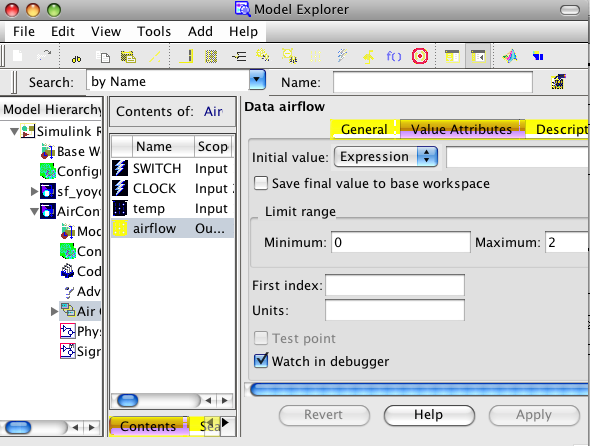
\includegraphics[width=11cm]{modelExpl}
\caption{Model explorer}
\label{model}
\end{figure}

\paragraph{Simulink Function}~\\
A Simulink function is a graphical object that you fill with Simulink blocks and call in the
actions of states and transitions. It behaves like a function-call subsystem block of a Simulink
model. If the function is in a state, it can be called in that state and all its
substates; if it is in the chart, it can be called anywhere in the chart. When the state is entered
(exited), the function is enabled (disabled).

These are the steps to define a Simulink Function in a Stateflow:
\begin{itemize}
\item Add a Simulink function by draging the icon 
\includegraphics[width=.6cm]{addFcn} from the
	Stateflow Editor toolbar on the left;	
\item Enter the function signature (function name {\tt simfcn}, formal argument names {\tt a\_i} 
	and return values {\tt r\_i}):\\
	{\tt [r\_1, r\_2,..., r\_n] = simfcn(a\_1, a\_2,..., a\_n)}\\
	The result will be this: \\
	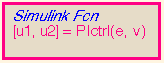
\includegraphics[width=2.5cm]{blockFcn}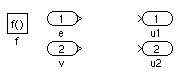
\includegraphics[width=3.5cm]{bFcn}\\
	To rename the function click the function box in the Stateflow Editor;
\item Define the elements of the Simulink function (don't delete the trigger port \fbox{{\tt f(c)}})
\item Configure the Input and Output ports of the Simulink function (double-click on the port).
\end{itemize}

In this example, to see the values of {\tt PID\_TRESH}, open {\tt Model Explorer}
(see fig.~\ref{model}), click on {\tt sf\_slswitch\_exemple} in {\tt Model Hierarchy}. 
Now click on {\tt Base Workspace} on {\tt Model Hierarchy} to change the value. 
The way the stateflow is updated: {\tt Model Explorer}, click on SwithcingController, 
update method = Inherited.
 
\vspace{.3cm} \noindent
Remark: for using the same step of the solver: file/Chart Properties/Updated method = Inherited\\
Update=Discrete (sample time: f(clock)); keep the clock when a code must be generated
(it is like a hardware interruption).\\
For continuous part (satellite) use the solver ode45.

\end{document}
